\documentclass[12pt]{article}
 
 %-Packages
\usepackage[margin=1in]{geometry} 
\usepackage{titlesec}
\usepackage{hyperref}
\usepackage{xcolor}
\usepackage{lmodern}
\usepackage[pagestyle]{titlesec}
\usepackage{tocloft}
\usepackage{graphicx}
\usepackage{lscape}



%-Counters
\newcounter{problem} \setcounter{problem}{1}
\addtocounter{section}{1}


%-Commands
\newcommand{\actionlog}[1]{\paragraph{Action Log ID: \theproblem\ -}{#1} ~\\ \addtocounter{problem}{1}}
\newcommand{\newweek}[1]{\underline{\section{Assignments - Week \thesection}}\\[5mm]}
\newcommand{\intention}[1]{\textbf{Intention:}{\textnormal\ #1} \newline}
\newcommand{\action}[1]{\textbf{Action:}{\textnormal\ #1} \newline}
\newcommand{\result}[1]{\textbf{Result:}{\textnormal\ #1} \newline}
\newcommand{\solution}[1]{\textbf{Solution:}{\textnormal\ #1} \newline}
\newcommand{\learning}[2]{\item \textit{#1} \textnormal{#2}}
\newcommand{\remember}{\paragraph{Key Points to Remember:}}
\newcommand{\question}[1]{\paragraph{Question: {\textnormal{\textit{#1}}} ~\\}}

%-Config

\definecolor{hyperblue}{RGB}{67, 69, 137}
\hypersetup{
    colorlinks,
    citecolor=black,
    filecolor=black,
    linkcolor=hyperblue,
    urlcolor=black,
    linktoc=all
}
\titleformat{\section}{\normalfont\Large\bfseries}{}{0em}{}
\renewcommand\numberline[1]{}

\title{Learning Journal}
\author{Aaron Hammond\\
FOAR705 - Digital Humanities}
\date{Semester 2, 2019}

%---------------------------------------------------------------
\begin{document}
%---------------------------------------------------------------

\begin{titlepage}
\maketitle
\vspace{-1.5cm}
\def\contentsname{\empty}
\tableofcontents
\end{titlepage}

%---------------------------------------------------------------Week 2

\newweek


\subsection{Formatting data tables in Spreadsheets}
\linebreak

\textit{1.What are some common challenges with formatting data in spreadsheets and how can we avoid them?}\\
\\
The largest challenge with spreadsheets is formatting the information in a manner in which the information can be easily read regardless of who looks at it. The spreadsheet should be written that no prior knowledge is required to decode the information inside it. This means restricting the use of colours or any sort of coding device and instead extend the data table to include the additional information.\\
\\
Exercises:\\
\textit{1. Identify what is wrong with this spreadsheet (SAFI messy). Discuss the steps you would need to take to clean up the two tabs, and to put them all together in one spreadsheet}\\
\begin{enumerate}
    \item Rename SAFI\_messy to SAFI\_raw
    \item Create a new spreadsheet titled SAFI\_0.1
    \item In a single spreadsheet copy and paste the information from Mozambique 
    \item Label the headings of the columns as follows A. country B. key\_id C. type\_roof D. type\_floor E. no\_rooms F. includes\_barn G. oxen H. poultry I. goats J. cows K. total\_livestock L. no\_plots M. water\_use N. comments (for cowshed, look after cows, only in summer, dead cows info)
    \item Organise the data according to the information as possible, consolidating as many lines as needed and using Cut+Copy functions to ensure no doubling of data or missing of information
    \item Copy data from Tanzania into the same spreadsheet (delete empty tab)
    \item Populate the country field while organise the data according to the same principles used for Mozambique
    \item Delete any obviously incorrect data (e.g. -999) and replace with (Null) value to indicate the information collected for this field is not entirely credible
    \item Save changes
\end{enumerate}
\textit{2. Discuss this data with a partner and make a list of some of the types of metadata that should be recorded about this dataset}\\
\begin{enumerate}
    \item Who attended these interviews?
    \item What does the use of liv mean in the columns?
    \item How often is \textit{frequently ?}
    \item Does months\_lack\_food mean no meals or not a sufficient number of meals?
    \item instanceID is used in what type of software?
\end{enumerate}

\subsubsection{Find examples of problem in data produced by your discipline}
Within my discipline of Anthropology, locating problem data is very difficult. Typically ethnographies are written using field notes that are supported by academic literature. In saying this it is very difficult to locate problem sets of data as the public typically and privy to them.

\subsection{Learning Journal \date{15/08/2019}} 
\vspace{5mm}

\actionlog{No Timestamp}
\begin{itemize}
    \item Intention: Create a line break in LaTeX
    \item Action: Used the Rich Text tab and pressed enter
    \item Result: No line break
    \item Improvements or Solutions: Researched and found command "newline" to assist with formatting.
\end{itemize}

\actionlog{No Timestamp}
\begin{itemize}
    \item Intention: Create a custom title for each page
    \item Action: Used the 'title' command and 'maketitle' in different combinations
    \item Result: No title added
    \item Improvements or Solutions: Instead use the title page function for the initial title and utilise 'sections' instead to group areas of my work.
\end{itemize}

\actionlog{No Timestamp}
\begin{itemize}
    \item Intention: Create a numbered bullet list
    \item Action: Used 'itemize' command
    \item Result: Bulletted list without numbers
    \item Improvements or Solutions: Instead utilise the enumerate command for numbered lists
\end{itemize}

\actionlog{No Timestamp}
\begin{itemize}
    \item Intention: Use the underscore in naming conventions
    \item Action: Quoted a filename which utilised the \_ character
    \item Result: Massive issues in formatting and text running off the page
    \item Improvements or Solutions: When using underscores the backslash command must be used before the \_ symbol to ensure formatting remains intact
\end{itemize}

\actionlog{No Timestamp}
\begin{itemize}
    \item Intention: Create a counter so i don't have to manually count my problems
    \item Action: Created a counter and attempted to use stepcounter to print and increase it's value by 1 
    \item Result: Step counter did not print any characters
    \item Improvements or Solutions: Instead i used the counter command and referenced it using 'thecounter' and increased its value by 1 using 'addtocounter'afterwards
\end{itemize}

\actionlog{No Timestamp}
\begin{itemize}
    \item Intention: Fix the formatting issues caused by ending lists with vspace
    \item Action: Added vspace to the first Problem\_ID
    \item Result: All Problem\_IDs after the first are aligned differently
    \item Improvements or Solutions: Perhaps using a command other than vspace for formatting
\end{itemize}

\clearpage

%------------------------------------------------------Week 3

\newweek{}

\subsection{Data Carpentry (Spreadsheets)}
\subsubsection{Date formats in spreadsheets}
\paragraph{Question: What year is shown in the year column?} ~\\
When adding data point '17/11' into the interview date column the Year column (formatted as =YEAR(A\$)) populates the field with '2019' (or the current year)
\newline
\paragraph{Key Points to Remember}
\begin{itemize}
    \item When working with dates within spreadsheets it is best to divide the three points of data into their own columns
    \item Do not allow the software to store the information as dates but integers instead to ensure they can be translated correctly to other software
    \item Excel will store dates as the current year unless specified otherwise
\end{itemize}

\subsubsection{Quality Assurance}

\paragraph{Key Points to Remember}
\begin{itemize}
    \item Data Validation tools help to mitigate errors and provide restrictions on the type of data that can be placed into columns
    \item Error messages can be customized as warnings or hard stops.
    \item Drop-down lists can be created per each data validation rule or can be sourced from within the document
    \item Overuse of these could cause issues if encountering unexpected  conditions or unique circumstances 
\end{itemize}

\subsubsection{Exporting Data}
\paragraph{Key Points to Remember}
\begin{itemize}
    \item File formats such as .xls and .xlsx are proprietary format and risk not being supported by future technology
    \item To ensure a document is more timeless and usable within a range of software, data should be saved as a .csv (comma seperated values) file type
    \item Within csv files ensure that any commas used in data fields are written within double-quotation marks to ensure that data is not reformatted incorrectly on re-opening
    \item Because it is formatted simply with commas and lines, .csv files can be edited in any text edit (such as notepad)
\end{itemize}

\subsection{Learning Journal}

\subsubsection{New Techniques and Commands Learned:}
\begin{itemize}
    \learning{subsubsection}{can be used to keep effective formatting within a subsection}
    \learning{tilde+doublebackslash}{can be used to force a line break after the paragraph command}
    \learning{verb}{can be used to ignore coding commands}
    \learning{newcommand[]}{can be used to create macros and within brackets you specify how many arguements you would like to include, arguments are referenced with the 'pound sign + number' combination}
    \learning{setcounter}{is used to set the value of a counter by specifying the counter name and the value within two separate curly bracket sets}
    \learning{backslash+space}{can be used to force a space}
    \learning{the+countername}{is the command to print the counter's value}
\end{itemize}

\subsubsection{Action Log}

\actionlog{22/08/2019 15:21}
\intention{Neatly format within a Subsection}
\action{attempted to use paragraph command to a standardized formatting}
\result{new line did not include referencing numbers for location}
\solution{Use the subsubsection command instead}

\actionlog{22/08/2019 15:36}
\intention{Write the cell variable from excel into Overleaf using the \$ symbol}
\action{Write the symbol as i would have any other}
\result{remaining code was highlighted in red indicating there was something missing or the code wouldn't recompile correctly}
\solution{Use the backslash character before the \$ to ensure it prints correctly}

\actionlog{22/08/2019 15:43}
\intention{Use the paragraph command to introduce and emphasize text then continue with normal text underneath}
\action{Attempted the paragraph command followed by \textit{newline} command however no return was created}
\solution{I utilized the \textit{tilde+double-backslash} command to force a new line}

\actionlog{22/08/2019 15:53}
\intention{Create a new command that automatically formatted the 'Things that i learned' area - having the command and it's action using differently formatted text}
\result{All the text came through \textit{italic}}
\solution{When creating a new command ensure to select the correct number of arguments in the first bracket}

\actionlog{22/08/2019 16:32}
\intention{Print a counter's value by referencing its name}
\action{Within the \textit{newcommand} for action logs I wrote the counter's name to be referenced}
\result{Counter was not printed}
\solution{In order to print a counter it must be preceded by \textit{the} e.g. If your counter is named dinosaur it mus be printed by typing \textit{thedinosaur}}

\actionlog{22/08/2019 16:56}
\intention{Create a new counter that inherently had a value of 1}
\action{Used the \textit{newcounter} command and placed the value that I wanted in the following bracket}
\result{Counter didn't appear when I attempted to print it}
\solution{The bracket isn't to dictate a value for the counter but what section it corresponds to, a second command of \textit{setcounter} must be used to explicitly set it}

\actionlog{22/08/2019 17:11}
\intention{Simply add a space after inserting a printed counter}
\action{Added an extra space after printing it with 'theproblem'}
\result{No space was added}
\solution{In order to ensure an additional space is added i used the \textit{backslash+space} command to force it there}

\actionlog{22/08/2019 17:41}
\intention{Print what is specifically written in the code}
\action{I placed the text that i wanted printed within quotation marks and insert brackets}
\result{It created bizzarre characters and was not at all what i wanted}
\solution{I can use the \textit{verb} and utilize | marks to print without translating the commands}
\newpage

%---------------------------------------------------------Week4
\newweek{}
\subsection{Data Carpentry (Shell)}
\subsubsection{Introducing the Shell}
%Shell1
\question{What is a command shell and why would I use one?}
A shell is a text-based command line interface that responds explicitly to commands entered. This type of interface is useful when conducting highly-repetitive tasks and as a terminal to send commands to a remote machine.  
\remember
\begin{itemize}
    \item Shell's main advantage is to increase the action-to-keystroke ratio by automating repetitive tasks
    \item \textit{ls} command can be used to list files within the current directory
    \item \textit{cd} command can be used to change directory
\end{itemize}
%Shell2
\subsubsection{Navigating Files and Directories}

\question{Starting from /Users/amanda/data, which of the following commands could Amanda use to navigate to her home directory, which is /Users/amanda?}
Amanda would need to use the \textit{cd \~} command

\question{Using the filesystem diagram below, if pwd displays /Users/thing, what will ls -F ../backup display?}
4. original/ pnas\_final/ pnas\_sub/

\question{Using the filesystem diagram below, if pwd displays /Users/backup, and -r tells ls to display things in reverse order, what command(s) will result in the following output}


\question{How can I move around on my computer?}
The command \textit{cd} is used to move around the computer.

\question{Can I see what files and directories I have?}
The command \textit{ls} will list the files and filders within a the specified folder. If no folder is specified the currently occupied folder items will be displayed.

\question{How can I specify the location of a file or directory on my computer?}
This can be achieved by using the -F option and dictating the folder location e.g. \textit{ls -f users/aaron/documents}

\remember
\begin{itemize}
    \item \textit{pwd} command can be used to print the current working directory
    \item \textit{ls --help} command will list all the options for the ls command
    \item \textit{cd \~, .. or -} Tilde goes home, .. goes up and - goes back
    
\end{itemize}

\subsubsection{Working With Files and Directories}

\question{How can I create, copy, and delete files and directories?}
Command \textit{mkdir} can be used to create a folder \\
Command \textit{touch <filename>} can be used to create a blank file \\
Command \textit{mv} will move desired file(s) to specified location
Command \textit{cp} will copy desired files to specified location (if same location it will be copied and renamed)
Command \textit{rm} will delete a file, use -r option to delete a directory and -i for a prompt

\question{When might you want to create a file this way? (using touch command}
The file size is 0kb and it could be used when running loop commands or to quickly store data in a file using a script.

\question{Fill in the blanks to move these files to the current folder (i.e., the one she is currently in):}
\$ mv ../analyzed/sucrose.dat ../analyzed/maltose.dat .

\question{After creating and saving this file you realize you misspelled the filename! You want to correct the mistake, which of the following commands could you use to do so?}
mv statstics.txt statistics.txt

\question{What is the output of the closing ls command in the sequence shown below?}
2.recombine

\question{What happens when we execute rm -i thesis\_backup/quotations.txt? Why would we want this protection when using rm?}
This will provide a prompt forcing you to enter another command to delete the file.

\question{In the example below, what does cp do when given several filenames and a directory name?}
This will copy the two files into the destination folder (backup)

\question{In the example below, what does cp do when given three or more file names?}
Command cannot be executed as the file is not a location.

\question{When run in the molecules directory, which ls command(s) will produce this output?}
ls *t??ne.pdb

\question{The fructose.dat and sucrose.dat files contain output from her data analysis. What command(s) does she need to run so that the commands below will produce the output shown?}
Question already states that fructose.dat and sucrose.dat are in the analyzed folder. But if you would like to move them elsewhere you would use mv *.dat followed by your location

\question{Which of the following set of commands would achieve this objective? What would the other commands do?}
$ mkdir 2016-05-20\\
$ mkdir 2016-05-20/data\\
$ mkdir 2016-05-20/data/processed\\
$ mkdir 2016-05-20/data/raw\\
\\
Would create the desired folder structure.

\question{How can I edit files?}
Text files can be edited by using the nano command or renamed using the \textit{mv} command

\subsection{Learning Journal}
\subsubsection{New Techniques and Commands Learned:}
\begin{itemize}
    \learning{0mm}{Can be used to apply vspace without the command}
    \learning{rule}{Command can be used to rule a line accross the page}
    \learning{empty}{Value can be used to empty a default field (e.g. contentsname}
    \learning{asteriks}{At the end of a command (such as section) can be used to prevent it from including a number}
    \learning{hypperref}{Package can be used to link the table of contents to its location within the document}
    \learning{xcolor}{Package can be used to create custom colours for reference}
\end{itemize}

\subsubsection{Action Log}

\actionlog{29/08/2019 14:27}
\intention{Place a border around the title page in elaboration I}
\action{Attempted to use the \textit{frame} command around title page}
\result{Everything was removed except the data within a small frame}
\solution{Found code that helped me format my title page correctly \hyperlink{https://tex.stackexchange.com/questions/407812/page-border-for-cover-page-in-latex?rq=1}{here}} 

\actionlog{29/08/2019 14:58}
\intention{Remove the word contents from the Table of Contents command}
\action{Tried toc and table commands in the hopes that would remove it}
\result{Contents header was still printed}
\solution{I found another person with a similar issue and their solution was to use the \textit{def} command to define the contentsname variable to empty. Code found \hyperlink{https://latex.org/forum/viewtopic.php?t=8151}{here}.}

\actionlog{29/08/2019 18:04}
\intention{To remove the number before each section}
\action{Remove the begin section commands and replace them with just section* commands}
\result{The numbers were removed from the headers but unfortunately from the table of contents too}
\solution{Find a way to simply hide the numbers instead of removing them}

\actionlog{29/08/2019 18:11}
\intention{Hide the section numbers}
\action{Replace the section* commands with just section and introduce variable setcounter secnumdepth to 0}
\result{All numbers removed from all sections, not just Section}
\solution{Renew the section command only to prevent subsequent changes}

\actionlog{29/08/2019 18:30}
\intention{Add hyper reference links to the table of contents}
\action{Added the hyperref package and set the link colour to blue}
\solution{Worked correctly but links were too blue}

\actionlog{29/08/2019 23:30}
\intention{Create a new colour for referencing}
\action{Added package xcolor and used definecolor command using name,RGB,<R, G, B> then used newcolor name in hyperref parameters}
\result{A duller blue hyperlink}

\actionlog{29/08/2019 23:30}
\intention{Create a hyperlink to a URL}
\action{Used the \textit{hyperlink} command placing the label in the first argument and the link in the second}
\result{The label was the link and the URL was simply "here"}
\solution{Reverse the two arguments so clicking "here" takes you to the URL}
\newpage

%----------------------------------------------------------------Week 5
\newweek{}

\subsection{Data Carpentry (Unix Shell)}
\subsubsection{Pipes and Filters}
\question{What does \textnormal{>>} mean?}
The operator >> will print text as an addition to the files contents and not replace what is currently there.
\question{After the commands that correspond to the file animals-subset.txt:}
As the two commands use different operators the file will print the first three lines of animals.txt to the subset.txt - and then append it with the last two lines of animals.txt
\question{In order to find the 3 files which have the least number of lines in our directory - what command(s) would we need to run?}
wc -l * | sort-n | head -n 3
\question{What passes through each of the popes and the final redirect in the pipeline below?}
\begin{verbatim}
    cat animals.txt | head -n 5 | tail -n 3 | sort -r > final.txt
\end{verbatim}
This command will display the contents of the file animals.txt, print the first 5 lines, the next pipe will then filter to only print the last 3 lines of the 5 printed. Then the command will sort them in reverse order and save the results to the final.txt file
\question{Using uniq and another command, how can you list the animals without duplicating their names?}
The following command would achieve this
\begin{verbatim}
    cut -d , -f 2 animals.txt | sort | uniq
\end{verbatim}

\question{What command to produce a table that shows the total count of each type of animal in the file}
\begin{verbatim}
    cut -d , -f 2 animals.txt | sort | uniq -c
\end{verbatim}

\question{Can you match the same set of files with basic wildcard expressions?}
Yes just executing one command for A files and one for B
\question{Which of the following would remove only all the processed data files?}
\begin{verbatim}
    rm *.txt
\end{verbatim}

\subsubsection{Loops}
\question{Why do the commands have different outputs?}
One command will print the same thing for each file that matches the criteria. The other uses a variable allows it to loop and print the variable value once each

\question{What will be the output of the loop using c*?}
This will run the loop only on files beginning with c - and therefore will only displace cubane.pdb
\question{What is the effect of this loop? (Part 1)}
This will print the name and the contents into a file named alkanes. The last file processed will be the contents of alkanes.pdb (pentane.pdb)
\question{What is the output of this loop (Part 2)}
All the text from the .pdb files will be stored sequentially in the all.pdb file
\question{Dry Run Loop - do we want to run the command with weird quotation marks or not?}
We want to run Version 1 - version 2 will print the same thing for each file.\\
Edit: actually it appears the second version works - and will print the whole command within the command line
\question{Nested Loops: What would the following code do?}
The code will make 12 directories, each is named with two variables, the species and the temperature
\subsubsection{Shell Scripts}
\question{Write a script that takes any number of file names as command-line arguments}
I wrote a script 
\begin{verbatim}
    cut -d , -f 2 "$1" | sort | uniq
\end{verbatim}
But this didn't achieve all the files, i looked at the solution and should have added the loop and \$@ to ensure that it would repeat for all the different files present in the folder

\question{Why is history command listed in the history list?}
Because it was the last command that was executed. It can't run the history command without running it and logging it to history.

\question{Variable in Shell Scripts - What would i expect to see with a wildcard name and two arguments in a command}
In this instance i would expect to see the first and last line of each pdb file in the directory (if not an error from the quotation marks?)
\question{Write a script that takes the name of a directory and filename extension as its arguments}
To achieve this the script must use the wc command alongside two arguments and sorting to produce the correct result. The last two of the file are taken (as the last line is Total) and then you choose the head of the two.

\begin{verbatim}
    wc -l \$1/*.\$2 | sort -n | tail -n 2 | head -n 1
\end{verbatim}

\question{What would each script do?}
Script 1 - would print all the files in the current folder\\
Script 2 - would display the contents of 3 specified files \\
Script 3 - would print all pdb files that

\question{Debugging - what is wrong with the script?}
The variable is spelled incorrectly, should be \$datafile.

\subsubsection{Finding Things}
\question{Which command would result in the following output - and the presence of absence}

The command with the -w option, to prevent other words with 'of' letters in there
\question{Put these commands and pipes in the correct order}
\begin{verbatim}
    grep -w $1 -r $2 | cut -d : -f 2 | cut -d , 0f 1,3 > $1.txt
\end{verbatim}

\question{Using a for loop, how would you write a script that counts the number of each girls' name in the book?}
Script would need to perform 4 loops, one for each girls name through the same text which yields a single numbered result for each
\begin{verbatim}
    for girl in Jo Meg Beth Amy
    echo $girl
    grep -w $girl LittleWomen.txt | wc -l
    done
\end{verbatim}

\question{Matching and Subtracting - how to remove results with a second parameter?}
Easiest way is to filter the results again by using the v option.
\begin{verbatim}
    find data -name '*s.txt' | grep -v net
\end{verbatim}

\question{Write a short comment on the script}
It will return with all the .dat files and sort them by their number of lines 

\question{How to write a single search criteria for type, time of modification and user}
The script would need to match the files -type, modified within 1 day (mtime) and -user
\subsection{Learning Journal}

\subsubsection{New Techniques and Commands Learned:}

\paragraph{Overleaf}
\begin{itemize}
\learning{justify}{environment can be used instead of center to format the text evenly between margins}
\learning{href}{command should be used instead of \textit{hyperlink} to embody the link within text}
\learning{lmodern}{package can be used so symbols appear correctly instead of upside down question marks}
\end{itemize}
\paragraph{Unix Shell}
\begin{itemize}
\learning{wc}{command is used to count words, lines or characters of a file}
\learning{sort}{command can be used to order results}
\learning{head tail}{commands can be used to display the first and last records of a file}
\learning{cat}{used to display the contents of a file}
\learning{|}{can be used to write new commands that utilise the results of the previous}
\learning{variables}{in loops can be referenced with \$VAR}
\learning{for}{is the beginning of a loop, and must finish with done command}
\learning{quotation marks}{are used if values may have spaces in them}
\learning{\$@}{is used in scripts to execute on all potential files}
\learning{bash}{command is used to execute scripts}
\learning{grep}{command is used to search for words within files}
\learning{find}{command is used to find files}
\end{itemize}

\subsubsection{Action Log}
\actionlog{05/09/2019 12:56}
\intention{Used the hyperlink command in Overleaf to link text to a URL}
\action{Clicked the link}
\result{Took me to the table of contents}
\solution{Use the HREF command instead of hyperlink}

\actionlog{05/09/2019 13:47}
\intention{Format text as justify}
\action{Removed the center command and replaced it with justify}
\result{No formatting change took place}
\solution{Set the environment as justify instead of just a command, begin justify}

\actionlog{05/09/2019 22:30}
\intention{Write greater than symbols}
\action{Used these symbols as text}
\result{Displayed as upside down question marks}
\solution{Need to use package lmodern for symbols to be displayed correctly}


\actionlog{06/09/2019 00:20}
\intention{Write a script in Unix Shell}
\action{Wrote a loop script using the for command}
\result{Received error 'unexpected end of file'}
\solution{Edit the script again and add 'done' at the end}

\actionlog{06/09/2019 01:19}
\intention{Find a file in Unix Shell}
\action{Used command find . '*.txt'}
\result{Error: no such file or directory exists}
\solution{I needed to specify i was searching for the name, find . -name}

\actionlog{05/09/2019 23:53}
\intention{Write loop script for word count}
\action{Wrote script with looping and variable}
\result{Execution would just hang}
\solution{The variable was spelt incorrectly in the 3rd reference within the script}

\actionlog{05/09/2019 14:22}
\intention{Upload audio file for transcription}
\action{Uploaded my AAC file}
\result{oTranscriber says it's not supported by my browser}
\solution{Converted the file to a .wav and tried again}
\newpage
%------------------------------------------------------------------
\newweek{}
\subsection{Data Carpentry (OpenRefine)}
\subsubsection{Introduction}
\begin{itemize}
    \item OpenRefine provides a set of tools allowing the identification and amending of data
    \item All actions are easily reversed in OpenRefine
    \item Saving your work will be in a new file to allow for version history
    \item OpenRefine logs all the steps taken and allows them to be applied to other datasets (but does not modify the original dataset)
\end{itemize}

\subsubsection{Working with OpenRefine}
\question{Try sorting this facet by name and by count. Do you notice any problems with the data? What are they?}
The facet presents information regarding all the fields of that volumn (Village column). It has a record for each of the different values within the column. The values can be sorted alphabetically or by the number of times they appear in the list (their count)
\newline
Some errors appear to be:
\begin{itemize}
    \item ruca is likely a mispelling
    \item chirdozo is likely a mispelling
    \item 49 appears to be a placeholder of some sort
    \item 'Ruaca - Nhamuenda1' is incorrectly formatted with spaces instead
\end{itemize}

\question{Using faceting, find out how many different interview\_date values there are in the survey results}
There is a total of 19 different interview dates
\question{Is the column formatted as Text or Date?}
The column is formatted as text and not with numeric or date values
\question{Use faceting to produce a timeline display for interview\_date. You will need to use Edit cells, Common transforms, To date, in to convert this column to dates.}
Done.
\question{During what period were most of the interviews collected?}
From 16/11/2016 to 04/12/2016 had the highest volume of interviews. More accurately though is the month of November 16' had the largest amount.
\question{What command would you use to remove the right bracket and apostrophes from the column of data?}
\begin{verbatim}
    value.replace(" ", "")
    value.replace("'", "")
    value.replace("]", "")
\end{verbatim}
\question{Which two items are the most commonly owned? Which are the two least commonly owned?}
The most common items owned are mobile phones and radios; the fewest owned items are cars and computers
\question{Which month(s) were farmers more likely to lack food?}
The months of October and November.
\question{Which were the common months without water?}
September and October
\question{What was the most common livestock owned?}
Oxen and Cows
\question{Most common responses for strategies for food mitigation}
Was lab\_ex\_food and na
\question{Most common responses for resolution change?}
Were nothing (null) or less work
\subsubsection{Filtering and Sorting with OpenRefine}
\question{What roof types are selected by this procedure?}
This feature will on show the rows that contain a value in the 'roof\_type' column that corresponds to what is entered into the filter/facet box
\question{How would you restrict this to only one of the roof types?}
By typing out the remaining feature of the roof you're after so the results are further refined. e.g. mabatisloping
\question{Use include / exclude to select only entries from one of these two roof types}
By mousing over the facet options on the left side you can elect to include or exclude rows that contain the desired/ undesired value.
\question{Sort the data by gps\_Altitude. Do you think the first few entries may have incorrect altitudes?}
Yes, as all the other values are above 600 I would assume that these 4 entries with a value of 0 are errors or mistakes.
\question{Can you tell from it’s GPS coordinates which village it belong to?}
It is most likely Chirodzo as the longitude values are very similar and have identical altitude values. 
\question{Is it the same village as when comparing GPS coordinates?}
Yes, now we can confidently say that because of all the matching criteria, village 49 is Chirodzo
\subsection{Learning Journal}
\subsubsection{New Techniques and Commands Learned:}
\paragraph{Overleaf}
\begin{itemize}
    \learning{vspace*}{can be used to force vspace after a new page command}
    \learning{titlesec}{package can be used to simply hide the numbering of sections but still retain its functionality}
    \learning{titleformat}{command can be used to alter the default formatting of certain types of text e.g. sections}
\end{itemize}
\paragraph{OpenRefine}
\begin{itemize}
    \learning{facets}{help give an overview of the data}
    \learning{transform}{features can be used to format columns into specific types of values e.g. from text to dates}
    \learning{clustering}{can be used to clean up errors in data entry instantly}
    \learning{value.replace}{as an expression can be used to find and replace values within the column}
    \learning{value.split}{can be used to explicitly state which symbol is used within the column to separate data values}
    \learning{A}{good distinction is that faceting gives you an overview description of all of the data that is currently selected, while filtering allows you to select a subset of your data for analysis}
\end{itemize}
\subsubsection{Action Log}

\actionlog{12/09/2019 14:04}
\intention{Remove section numbers from heading and table of contents}
\action{Added the titlesec package and defined sections using the titleformat command}
\result{Section numbering was removed successfully from headings and table of contents}
\solution{Using the code found \href{https://tex.stackexchange.com/questions/220566/sections-suppress-numbers-but-retain-title-in-header}{here} i could make the desired formatting changes}

\actionlog{12/09/2019 14:20}
\intention{Move the title up on the page to reduce the blank space above}
\action{Attempted to use the titling package with the setlength and droptitle commands}
\result{"Error: Option clash for package titlesec."}
\solution{Rather than use two conflicting packages vspace* could be used instead}

\action{12/09/2019 21:49}
\intention{OpenRefine: run multiple replace expressions together}
\action{Grouped the expressions all together as one replace action}
\result{Only the top expression functioned correctly}
solution{Need to use more sophisticated coding language for instance, group the commands together with additional .replace commands}
\newpage
%---------------------------------------------------------------------------------------

\newweek

\subsection{Data Carpentry (Open Refine)}
\subsubsection{Examining Numbers in OpenRefine}
\question{Transform three more columns, no\_members, yrs\_liv, and buildings\_in\_compound, from text to numbers. Can all columns be transformed to numbers?}
It's not possible to change Village into number values, only one was changed which was likely the mistake of village '49'
\begin{itemize}
    \item OpenRefine can be useful for maintaining numbered datasets
    \item All columns and data that is opened in OpenRefine is treated as text unless specified as otherwise
\end{itemize}
\subsubsection{Using scripts}
\begin{itemize}
    \item All the changes made in OpenRefine are logged and stored in JSON (Java Script Object Notation) format
    \item These scripts can be exported and pasted into other data sets as a means of replicating the same changes to a different data set
\end{itemize}
\subsubsection{Exporting and Saving Data from OpenRefine}
\question{After you have expanded the file look at the files that appear in this folder. What files are here? What information do you think these files contain?}
There is a history folder that holds the information regarding the changes made in open refine (probably the JSOR scripts). A data.zip file that contains the values for the data set and two JSON files that contain the pre and post metadata values.
\begin{itemize}
    \item Alternatively the cleaned data and transformed values can be exported as .csv files
    \item Exporting projects allows for them to be easily shared with others using OpenRefine, where they can see the raw data values and the changes you have made
\end{itemize}
\subsubsection{Other Resources in OpenRefine}
\begin{itemize}
    \item OpenRefine can also be used to fetch datasets from webservices such as geocoding grographic coordinates
    \item Also can be used to parse data from web sites by using a URL fetch feature
\end{itemize}

\subsection{Learning Journal}

\subsubsection{Action Log}
\actionlog{03/10/2019 14:12}
\intention{Convert PDF to text using texttopdf.exe}
\action{Double-clicked the exe}
\result{Blink of a command line then nothing}

\actionlog{03/10/2019 14:14}
\intention{Convert PDF to text using texttopdf.exe}
\action{Shift and Right clicked the explorer to open a powershell at the correct directory and executed}
\begin{verbatim}
    pdftotext.exe test1.pdf
\end{verbatim}
\result{Error: The term 'pdftotext.exe' is not recognized as the name of a cmdlet, function, script file, or operable program. Instead, i needed to try}
\begin{verbatim}
    .\pdftotext.exe test1.pdf
\end{verbatim}

\actionlog{03/10/2019 23:45}
\intention{Convert multiple PDF to text files using Powershell}
\action{Attempted to use the 'Get-childitem' -path -filter \*.pdf | foreach-object pdftotext}
\result{Multiple instances of the pdftotext command options. My command was missing the syntax and couldn't correctly execute the exe on the files, it just ran the exe without a target specified}
\solution{Research how to ensure that the exe runs on the files themselves without being specifically typed in the script\\
Alternatively, a simpler but manual process is to highlight the file and drag and drop on the exe, does everything but move the files}

\actionlog{04/10/2019 00:33}
\intention{Paste text into Cygwin64 Terminal}
\action{Selected and Ctrl+C to copy the text, and in the window attempted Ctrl+V}
\result{Nothing was pasted, just V}
\solution{In this program I needed to use shift and insert to paste in text}

\actionlog{04/10/2019 00:33}
\intention{Install Mozilla Deepspeech with Cygwin64 Terminal}
\action{Pasted text pip3 install deepspeech and executed}
\result{-bash: pip3: command not found}
\solution{What i needed to type was:}
\begin{verbatim}
    sudo apt install python3-pip
\end{verbatim}
Before i can install deepspeech.

\actionlog{04/10/2019 00:46}
\intention{Use Alveo to test speech to text}
\action{Attempst to navigate the website and use the tool showcased that you can't simply transcribe your own files}

\actionlog{04/10/2019 02:00}
\intention{Use deepspeech to transcribe an audio file}
\action{Installed deepspeech and ran the documented commands}
\result{deepspeech command not found}
\solution{After some research it appears that deepspeech doesn't support the windows ubuntu terminal}

\newpage
%-------------------------------------------
\newweek

\subsection{Data Carpentry (R)}
\subsubsection{Before we Start}
\question{Use the install option from the packages tab to install the tidyverse package}
Click the install button - search for the package tidyverse and click OK
use the install.package("packagename")

\paragraph{Top Left: Source, of scripts and documents}
\paragraph{Bottom Left: Console, what R would look like and be like without RStudio}
\paragraph{Top Right: Environment/History, look at what changes you have made}
\paragraph{Bottom Right: Files, file browser to see the individual files within your project}


\subsubsection{Introduction to R}
\question{What do you think is the current content of the object area_acres? 123.5 or 6.175?}
The environment lists the value of area\_acres as 6.175 as the value was stored before the dependant variable was changed. Correct! So i would need to re-run the assign value command for it to be updated

\question{Show that changing the values of either length and width does not affect the value of area}
\begin{verbatim}
length <- 5, width <- 5, area <- length * width
length <- 2
area [1] 25
\end{verbatim}
\begin{verbatim}
    round(2.492321345, 2)
\end{verbatim}

\question{What other functions exist that are similar to round? How do you use the digits parameter in the round function?}
functions Signif, floor and trunc are all additional functions\\
You add another argument and divide them by a comma e.g.

\question{We’ve seen that atomic vectors can be of type character, numeric (or double), integer, and logical. But what happens if we try to mix these types in a single vector?}
I imagine that R will produce an error in response, or assigns all values to the characteristics of the first data type

\question{What will happen in each of these examples? (hint: use class() to check the data type of your objects):}
Classes would be, character, numeric, numeric and character

\question{How many values in combined_logical are "TRUE" (as a character) in the following example:}
num\_logical has 1\\
char\_logical has 1\\
combined)\_logical has 1 (the true in num\_logical gets converted into a 1 before it gets converted into "1" in combined\_logical

\question{Using this vector of rooms, create a new vector with the NAs removed}
\begin{verbatim}
    rooms <- c(1, 2, 1, 1, NA, 3, 1, 3, 2, 1, 1, 8, 3, 1, NA, 1)
    roomswona <- na.omit(rooms)
\end{verbatim}
\question{Use the function median() to calculate the median of the rooms vector.}
\begin{verbatim}
    median(roomswona) - median is 1
\end{verbatim}
\question{Use R to figure out how many households in the set use more than 2 rooms for sleeping}
\begin{verbatim}
    length(roomswona[roomswona > 2]) - answer is 4
\end{verbatim}

\subsection{Learning Journal}


\subsubsection{New Techniques and Commands Learned:}

\paragraph{R}
\learning{dir.create}{command to script the creation of directories}
\learning{download.file}{command can be used to retreive files from a URL}
\learning{install.package}{command can be used to install packages from the command line instead of the GUI}
\learning{alt + -}{will automatically format the assign value symbol}
\learning{\#}{is used to write comments for whatever follows it}
\learning{na.omit(vector}{can be used to create a new vector using the same data set but omitting the missing values}

\subsubsection{Action Log}

\actionlog{10/10/2019 23:11}
\intention{Script output from deepspeech into a text file}
\action{Added <variable > file.txt}
\result{No text file created}
\solution{Add the > command to the end of the original command to run deepspeech}

\actionlog{10/10/2019 23:18}
\intention{Create a file with the contents of the output - but use the original file name with a prefix}
\action{Using a for script in the unix shell i tried to simply add the prefix to the variable}
\result{
  interview\_/mnt/c/FOAr705/project/interviews/testwav11.wav.txt: No such file or directory}
\solution{create the file and run another command to rename it}

\actionlog{11/10/2019 00:43}
\intention{Move folder to a directory}
\action{typed mv mnt/c/foar}
\result{-bash: cd\\ mnt/dinosaur/village: No such file or directory}
\solution{I forgot the initial /}

\actionlog{11/10/2019 01:00}
\intention{Run a bash script within a bash script}
\action{After running the initial script i wanted to trigger another script to rename and move the files}
\result{mv: cannot stat '*.txt': No such file or directory
mv: cannot stat '*.txt': No such file or directory}
\solution{The directory must be set for where the new script will run, after adding a cd command the script found the necessary files}

\actionlog{17/10/2019 16:23}
\intention{Print the values of a vector that meet a criteria}
\action{Ran the command [roomswona>2]}
\result{Error unexpected [ in [}
\solution{i needed to establish the vector before trying to print it. the following worked instead\\
roomswona[roomswona>2]}
%--------------------------------------
\newpage

\newweek

\subsection{Data Carpentry (R)}

\subsubsection{Starting with Data}
\question{Create a data frame (interviews\_100) containing only the data in row 100 of the interviews dataset.}
I run the command, interviews\_100 <- interview(100,) which will place the value of row 100 to the interviews\_100 vector

\question{Create a new data frame (interviews_last) from that last row}
interviews\_last <- interviews[131,]

\question{Use nrow() to extract the row that is in the middle of the data frame. Store the content of this row in an object named interviews_middle.}
\begin{verbatim}
    norow <- nrow(interviews)
    interviews_middle <- interviews[(norow / 2), ]
\end{verbatim}
\question{Combine nrow() with the - notation above to reproduce the behavior of head(interviews), keeping just the first through 6th rows of the interviews dataset}
interviews\_head <- interviews[-(7:norow), ]
interviews\_middle <- interviews[(]
132), 1

\question{Rename the levels of the factor to have the first letter in uppercase: No,Undetermined, and Yes.}
\begin{verbatim}
    levels(memb_assoc) <- c("No","Undetermined","Yes")
\end{verbatim}
\question{Now that we have renamed the factor level to ]Undetermined, can you recreate the barplot such that Undetermined is last (after Yes)?}
\begin{verbatim}
    memb_assoc <- factor(memb_assoc,levels = c("No","Yes","Undetermined"))
plot(memb_assoc)
\end{verbatim}

\subsection{Learning Journal}

\subsubsection{New Techniques and Commands Learned:}

\paragraph{R}

\learning{factors}{can be used to place your data into categories}
\learning{:}{can be used to select only a particular range of the dataset}
\learning{nrow}{will provide a set number of rows}

\subsubsection{Action Log}

\actionlog{24/10/2019 16:27}
\intention{I tried to create a new data vector of top 100 rows using command}
\action{I ran the command interviews\_100 <- interviews[-c(1:100), ]}
\result{Returned the wrong information}
\solution{What i needed to use was interviews\_100 <- interviews[100, ]}

\actionlog{24/10/2019 16:48}
\intention{Read a csv file in R}
\action{ran command read(SAFI_clean.csv}
\result{Error: unexpected symbol in "read SAFI_clean.csv"}
\solution{Instead i needed to run the command}
\begin{verbatim}
    > read_csv("data/SAFI_clean.csv")
\end{verbatim}


\actionlog{24/10/2019 17:10}
\intention{Set a default directory for voyant server to automatically collect as a corpus}
\action{Edited the server-settings file and set the corpus as follows}
\begin{verbatim}
    uri_path = /?input=/localhost/file:///C:/foar705/project/ready/gat.txt
\end{verbatim}
\result{Voyant server just ran the analysis on the words in the file path}

\actionlog{24/10/2019 17:02}
\intention{Set a default directory for voyant server to automatically collect as a corpus}
\action{Edited the server-settings file and set the corpus as follows}
\begin{verbatim}
    uri_path = /?corpus=333.333 (to indicate a local corpus)
\end{verbatim}
\result{A corpus was specified but does not exist, could not be migrated and could not be recreated 333.333\\
java.lang.IllegalArgumentException: A corpus was specified but does not exist, could not be migrated and could not be recreated: 333.333}
%--------------------------------

\newpage
\newweek{}
\subsection{Data Carpentry (R)}
\subsubsection{Introducing dplyr and tidyr}
\question{Create a new data frame from the interviews data that meets the following criteria. Contains only the village column and a new column called total\_meals containing a value that is equal to the total number of meals served in the household per day on average. Only the rows where total\_meals is greater than 20 should be shown in the final data frame.}
\begin{verbatim}
    > newviews <- interviews %>% 
+     + mutate(totalmeals = no_membrs * no_meals) %>% 
+     + select(village, totalmeals) %>% 
+     + filter(total_meals>20)
\end{verbatim}

\question{How many households in the survey have an average of two meals per day? Three meals per day? Are there any other numbers of meals represented?}
\begin{verbatim}
> interviews %>% 
+     count(no_meals)
# A tibble: 2 x 2
  no_meals     n
     <dbl> <int>
1        2    52
2        3    79
\end{verbatim}
No, only 2 and 3 records.

\question{Use group\_by and summarize to find the mean, min, and max number of household members for each village. Also add the number of observations}
\begin{verbatim}
    > interviews %>% 
+     group_by(village) %>% 
+     summarize(
+         mean_no_membrs=mean(no_membrs),
+         min_no_membrs=min(no_membrs),
+         max_no_membrs=max(no_membrs),
+         n=n())
\end{verbatim}
\question{What was the largest household interviewed in each month?}
\begin{verbatim}
    > interviews %>% 
+     mutate(month=month(interview_date),
+            year=year(interview_date)) %>% 
+     group_by(year,month) %>% 
+     summarize(max_no_membrs=max(no_membrs))
# A tibble: 5 x 3
# Groups:   year [2]
   year month max_no_membrs
  <dbl> <dbl>         <dbl>
1  2016    11            19
2  2016    12            12
3  2017     4            17
4  2017     5            15
5  2017     6            15
\end{verbatim}

\question{Create a new data frame that has one column for each month and records TRUE or FALSE for whether each interview respondent was lacking food in that month.}
\begin{verbatim}
    interviews_months_lack_food <- interviews %>%
  separate_rows(months_lack_food, sep=",") %>%
  mutate(months_lack_food_logical  = TRUE) %>%
  spread(key = months_lack_food, value = months_lack_food_logical, fill = FALSE)
\end{verbatim}

\question{How many months (on average) were respondents without food if they did belong to an irrigation association? What about if they didn’t?}
\begin{verbatim}
    > interviews_months_lack_food %>%
+     mutate(number_months = rowSums(select(., Apr:Sept))) %>%
+     group_by(memb_assoc) %>%
+     summarize(mean_months = mean(number_months))
# A tibble: 3 x 2
  memb_assoc mean_months
  <chr>            <dbl>
1 no                2.31
2 yes               2.64
3 NA                2.95
\end{verbatim}
\newpage
\subsection{Learning Journal}

\subsubsection{New Techniques and Commands Learned:}

\paragraph{R}

\learning{select}{command to select what information to print or work with}
\learning{filter}{command to filter rows by a certain column value}
\learning{pipes}{can be used to run a set of commands (works very similar to unix)}
\begin{verbatim}
    Pipes can be used by %>% - shortcut is ctrl+shift+m
\end{verbatim}
\learning{!}{symbol can be used to indicate 'not equal to'}
\learning{read\_csv}{command can be used to open a csv file}
\learning{write\_csv}{can write new objects or data sets to a csv}
\learning{group\_by}{command can be used to group the results of rows together to understand some data more easily}
\learning{summarize}{can be used in conjunction with group\_by to focus on certain aspects of data}
\learning{mutate}{can be used to create new columns, which can refer to other columns data}

\subsubsection{Action Log}

\actionlog{31/10/2019 13:12}
\intention{Use a group and summarize command then add a filter}
\action{Ran the command}
\begin{verbatim}
    > interviews %>% filter(memb_assoc) %>% select(affect_conflicts,liv_count,no_meals) 
\end{verbatim}
\result{Error: Argument 2 filter condition does not evaluate to a logical vector}
\solution{filter command needed to ask for a criteria (memb\_assoc=YES)}

\actionlog{31/10/2019 13:17}
\intention{Create a new column based on an equation between other columns}
\action{Ran the following command}
\begin{verbatim}
    > interviews %>% 
+ mutate(people_per_room = no_members/rooms)
Error: object ' no_members' not found
> mutate(people_per_room = no_membrs/rooms)
Error in mutate(people_per_room = no_membrs/rooms) :
\end{verbatim}
\result{object no\_membrs not found}
\solution{Needed to set interviews as the dataset to work with}

\action{31/10/2019 13:25}
\intention{create a new column that multiplies one columns values with another}
\action{Ran the following command}
\begin{verbatim}
    > newviews <- interviews %>% 
+ mutate(totalmeals = no_membrs * no_meals) %>% 
+ select(village, total_meals) %>% 
+ filter(total_meals>20)
\end{verbatim}
\result{Result was the error}
\begin{verbatim}
    Error in .f(.x[[i]], ...) : object total_meals not found
\end{verbatim}
\solution{Use the correct object name, totalmeals}

\actionlog{31/10/2019 13:54}
\intention{Find min, max and mean of households grouped by village}
\action{Ran the following command}
\begin{verbatim}
    > interviews %>% 
+     group_by(village) %>% 
+     summarize(no_membrs,min(no_membrs),max(no_membrs))
\end{verbatim}
\result{Error: Column no\_membrs must be length 1 (a summary value), not 39}
\solution{Needed to change the syntax to}
\begin{verbatim}
      summarize(
      mean_no_membrs = mean(no_membrs),
      min_no_membrs = min(no_membrs),
      max_no_membrs = max(no_membrs)
\end{verbatim}

%---------------------------------

\newpage
\newweek{}
\subsection{Data Carpentry (R)}
\subsubsection{Data Visualisation with ggplot2}
\question{Use what you just learned to create a scatter plot of rooms by village with the respondent\_wall\_type showing in different colors. Is this a good way to show this type of data?}
\begin{verbatim}
    > ggplot(data = interviews_plotting, 
    aes(x = village, y = rooms)) +
+   geom_point(aes(color = respondent_wall_type))
\end{verbatim}
Not particularly, because so many of the plots want to occupy the exact same position it's hard to really gain much from the plot. Adding jitter would be more appropriate. However, even with jitter it is easy to confuse what plots are from what village.
\question{Replace the box plot with a violin plot}
\begin{verbatim}
    ggplot(data = interviews_plotting, 
    aes(x = respondent_wall_type, y = rooms)) +
    geom_violin(alpha = 0) +
    geom_jitter(alpha = 0.5, color = "tomato")
\end{verbatim}
\question{Create a boxplot for liv\_count for each wall type. Overlay the boxplot layer on a jitter layer to show actual measurements}
\begin{verbatim}
    ggplot(data = interviews_plotting, 
    aes(x = respondent_wall_type, y = liv_count)) +
    geom_boxplot(alpha = 0) +
    geom_jitter(alpha = 0.5)
\end{verbatim}
\question{Add color to the data points on your boxplot according to whether the respondent is a member of an irrigation association (memb\_assoc).}
\begin{verbatim}
    > ggplot(data = interviews_plotting, 
    aes(x = respondent_wall_type, y = liv_count)) +
+     geom_boxplot(alpha = 0) +
+     geom_jitter(alpha = 0.5)+
+     aes(color = memb_assoc)
\end{verbatim}
\question{Create a bar plot showing the proportion of respondents in each village who are or are not part of an irrigation association}
Need to create the dataset to plot before plotting.
\begin{verbatim}
    memb_count_village <- interviews_plotting %>% 
    filter(!is.na(memb_assoc)) %>% 
    count(village,memb_assoc) %>% group_by(village) %>% 
\end{verbatim}
Then plot the graph
\begin{verbatim}
    ggplot(memb_count_village, aes(x=village, y=n, fill=memb_assoc)) +
    geom_bar(stat = "identity", position = "dodge")
\end{verbatim}
The God village had the lowest number of people in an association.
\question{Experiment with at least two different themes. Build the previous plot using each of those themes. Which do you like best?}
I experimented with Void, Minimal and Light. Void and minimal are very similar but don't provide much information. Light is my preferred style.

\question{}
\begin{verbatim}
    ggplot(percent_items, aes(x=village, 
    y=percent, fill=village)) + 
    geom_bar(stat="identity",position="stack") +
    facet_wrap(~items) +
    theme_minimal() +
    scale_fill_brewer(palette="Spectral") +
    labs(title="Percent of respondents who own items",
         x="Village Name",
         y="Percent of Participants")
         ggsave("data_output/participant_items.png",
         width = 15, height = 10)
\end{verbatim}
\begin{landscape}
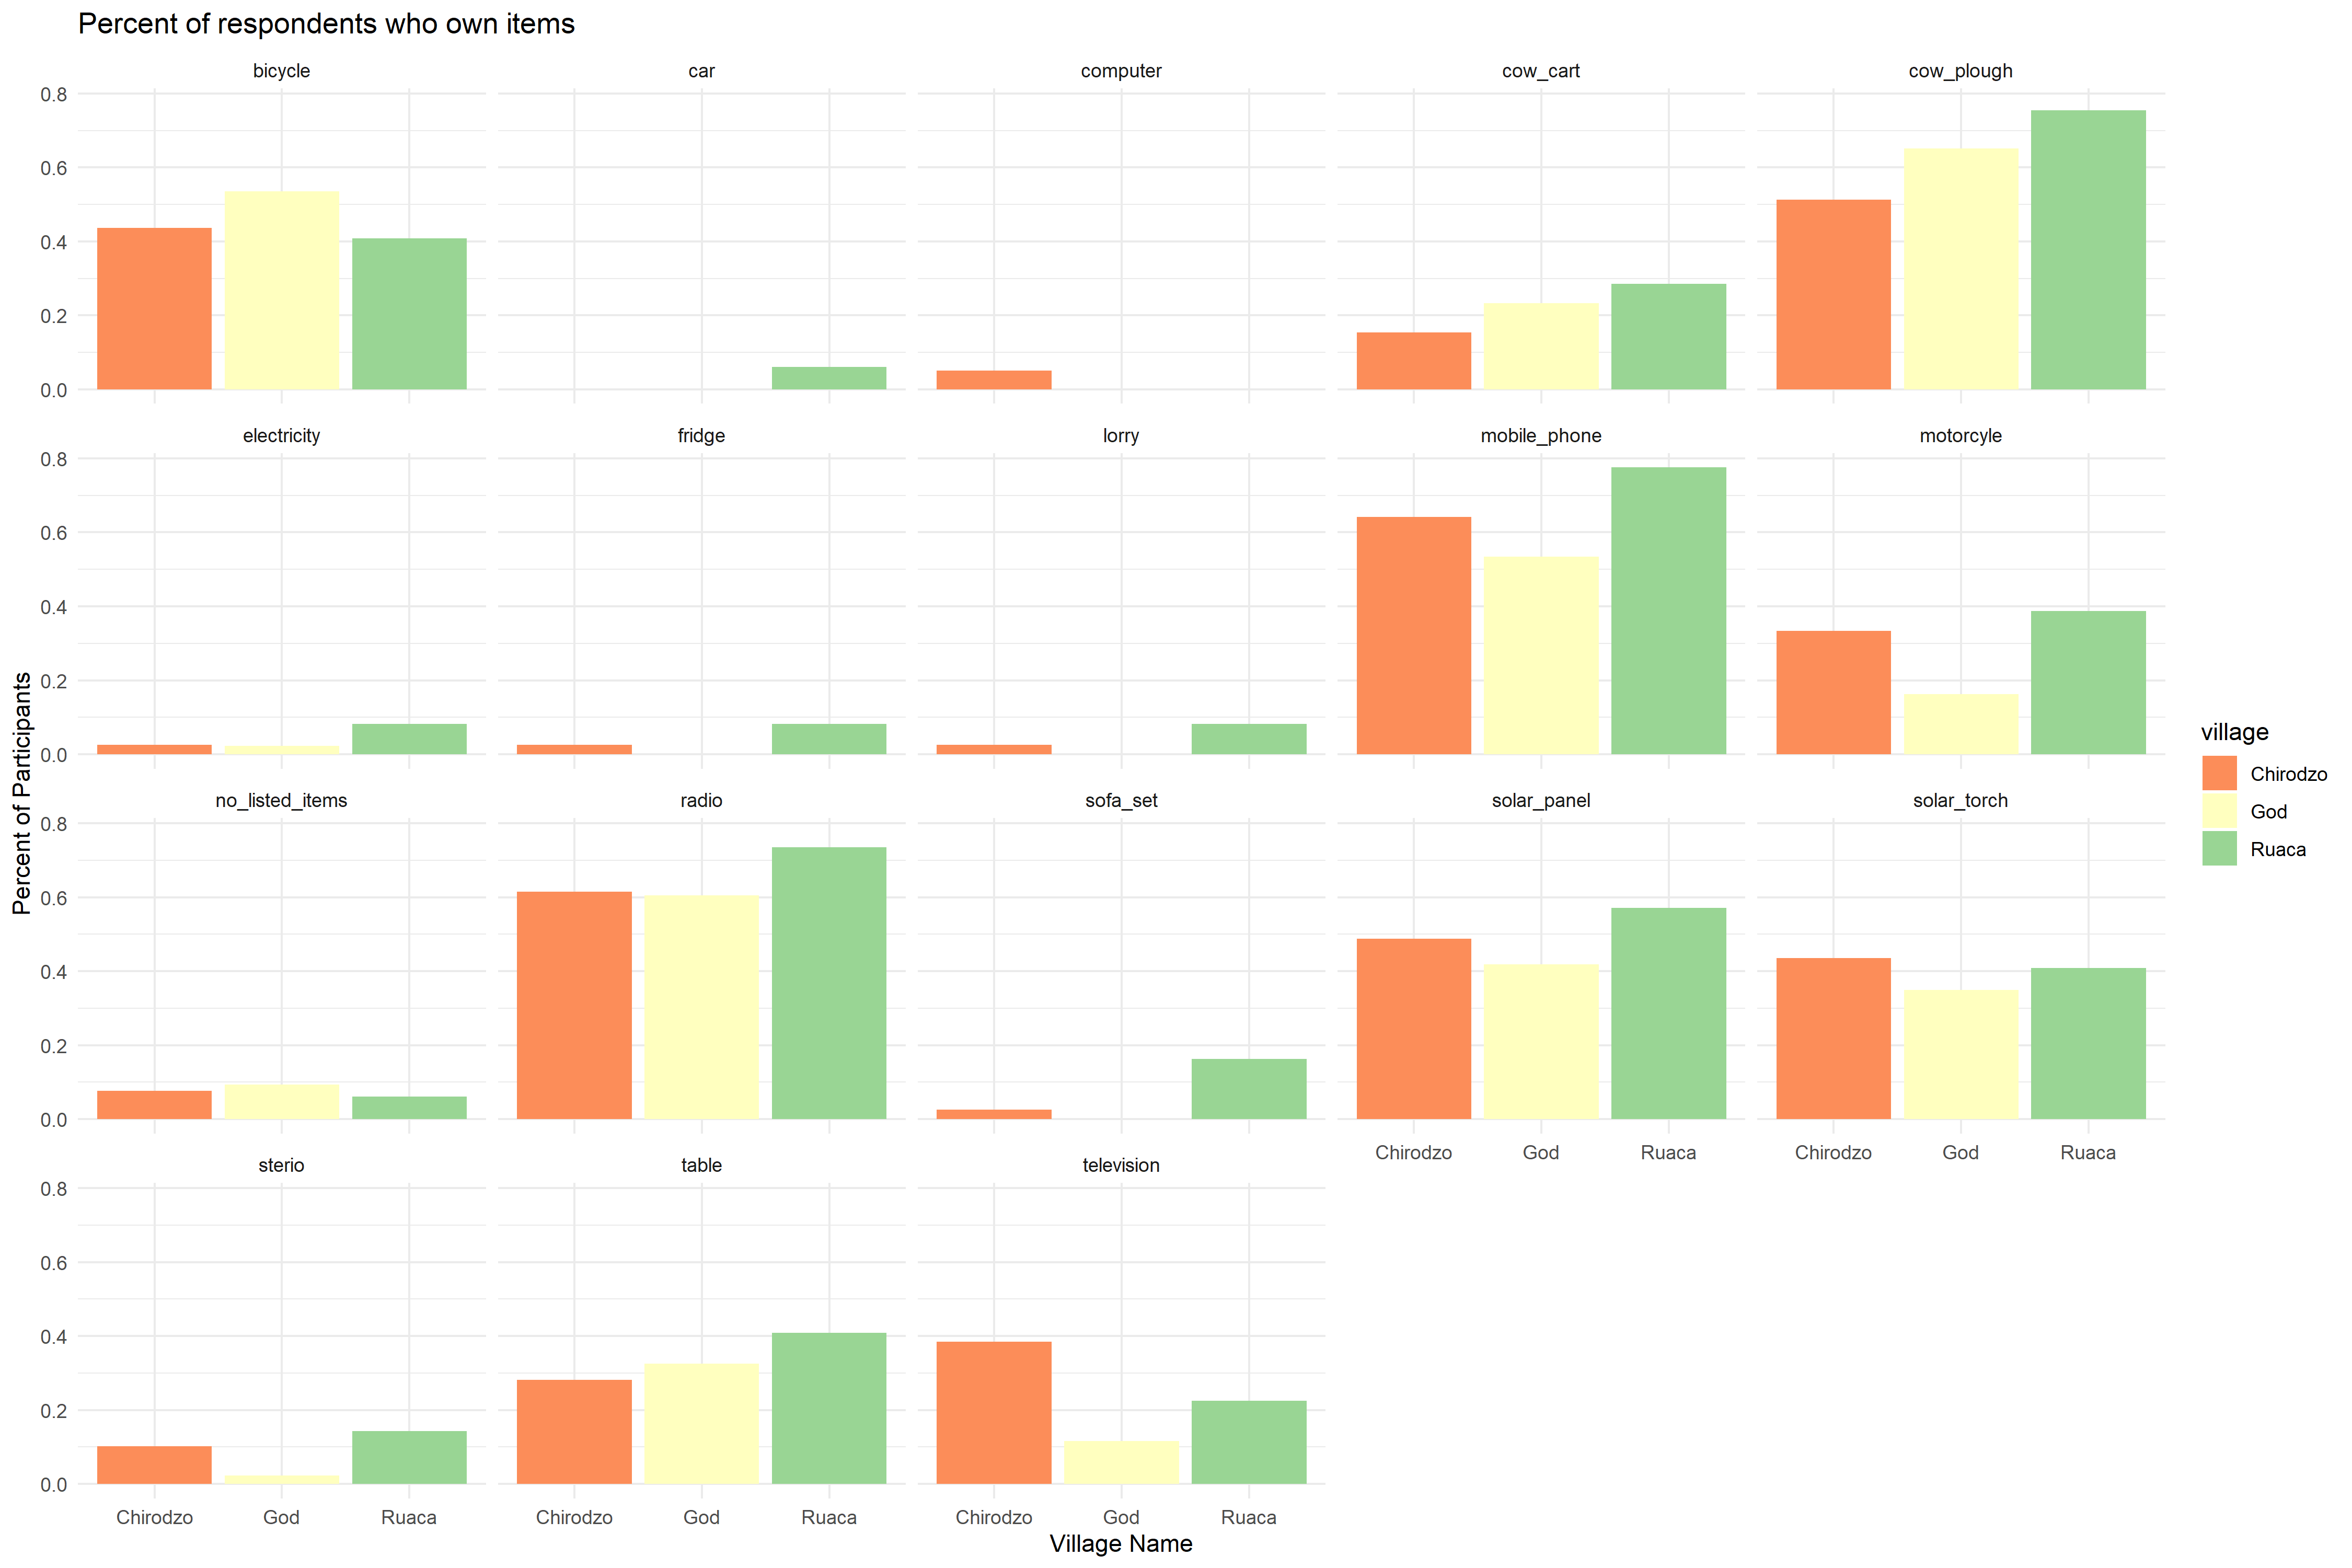
\includegraphics[scale=0.6]{participant}
\end{landscape}
\subsection{Learning Journal}

\subsubsection{New Techniques and Commands Learned:}
\paragraph{R}
\learning{plot}{command is used to determine the data used for a graph}
\learning{ggplot}{sets the aesthetics and settings of the graph and how the information is presented}
\learning{geompoint()}{creates a point based gragh}
\learning{facet}{allows you to generate multiple plots based on a categorical variable}

\subsubsection{Action Log}

\actionlog{31/10/2019 16:26}
\intention{Change the colour of only one aspect of the plots}
\action{I ran the following}
\begin{verbatim}
    > ggplot(data = interviews_plotting, 
      aes(x = respondent_wall_type, y = liv_count)) +
+     geom_boxplot(alpha = 0,) +
+     geom_jitter(alpha = 0.5)+
+     aes(color = memb_assoc)
\end{verbatim}
\result{All colours changed instead of just one}
\solution{Move the colour command to only one part of the plot. E.g.}
\begin{verbatim}
    jitter(alpha = 0, aes(color = memb_assoc))
\end{verbatim}
\actionlog{31/10/2019 16:46}
\intention{Plot wall type}
\action{I ran the following command in the console}
\begin{verbatim}
    > ggplot(percent_wall_type, 
    aes(x = village, y = percent, 
    fill = memb_assoc)) +
+     geom_bar(stat = "identity", position = "dodge")
\end{verbatim}
\result{Following error:}
\begin{verbatim}
    Error in FUN(X[[i]], ...) : object 'memb_assoc' not found
\end{verbatim}

\actionlog{31/10/2019 22:14}
\intention{Add a graphic to the document in Overleaf}
\action{Attempted to use the includegraphics command}
\result{No image inserted}
\solution{I need to import the includegraphics package}

\actionlog{31/10/2019 22:20}
\intention{See picture clearly and formatted correctly within the page}
\action{Used the includegraphics command}
\result{Picture's original dimensions were too big for the portrait page and couldn't be read with any clarity}
\solution{I imported the landscape package to place the picture in a landscape page as it better fits its aspect ratio}
\newpage
\newweek{}

\subsection{Learning Journal}
\subsubsection{Action Log}


\actionlog{07/11/2019 15:20}
\intention{Have voyant server automatically creata a corpus from a file hosted on cloudstor}
\action{Uploaded a file to cloudstor, created a public link and placed this into the serverconfig file}
\result{Due to javascript on cloudstor voyant server couldn't access the file}

\actionlog{07/11/2019 15:28}
\intention{Use a file hosted on iLearn as a corpus}
\action{Set the corpus as}
\begin{verbatim}
    https://ilearn.mq.edu.au/pluginfile.php
    /5795890/mod_resource/content
    /1/Sword%20-%20Finding%20Time%20to%20Write.pdf
\end{verbatim}
\result{Error: Failed attempt to create corpus}

\actionlog{07/11/2019 15:32}
\intention{Create a corpus with a file hosted by github}
\action{Edited the server config file to point to the following file}
\begin{verbatim}
    https://github.com/MQ-FOAR705/HammondA_Elaboration_II
    /blob/master/README.txt
\end{verbatim}
\result{Success, corpus loaded a single file successfully}

\actionlog{07/11/2019 15:36}
\intention{Load a corpus hosted by GitHub as a zip file}
\action{Uploaded a zip file filled with txt files as a corpus}
\begin{verbatim}
    https://github.com/MQ-FOAR705/HammondA_Elaboration_II
    /blob/master/ready.zip
\end{verbatim}
\result{Failed attempt to create corpus}


\end{document}